\pagebreak
\subsection{Manipulación}

A continuación vamos a experimentar con que tan manipulable es el algoritmo PageRank a medida que va cambiando el factor de teletransportacion. La idea es la siguiente, un algoritmo con un factor de teletransportacion bajo pondera menos en la matriz de transición el componente de la estructura del grafo. Por lo tanto, un Search Engine que tenga este factor de teletransportacion bajo va a ser sumamente manipulable, dado que puedo crear muchisimos nodos e inflar el ranking de cualquier sitio. Cuanto mayor es este factor, conjeturamos que vamos a observar que inflar cualquier sitio sera mucho mas costoso en termino de cantidad de sitios únicos que debo crear. De hecho, Page \& Brin en su paper consideran esto y mencionan que en Google se ponderan muchos factores para evitar lo que hoy se conoce como SEO (Search Engine Optimization).

\begin{figure}[H]
\centering
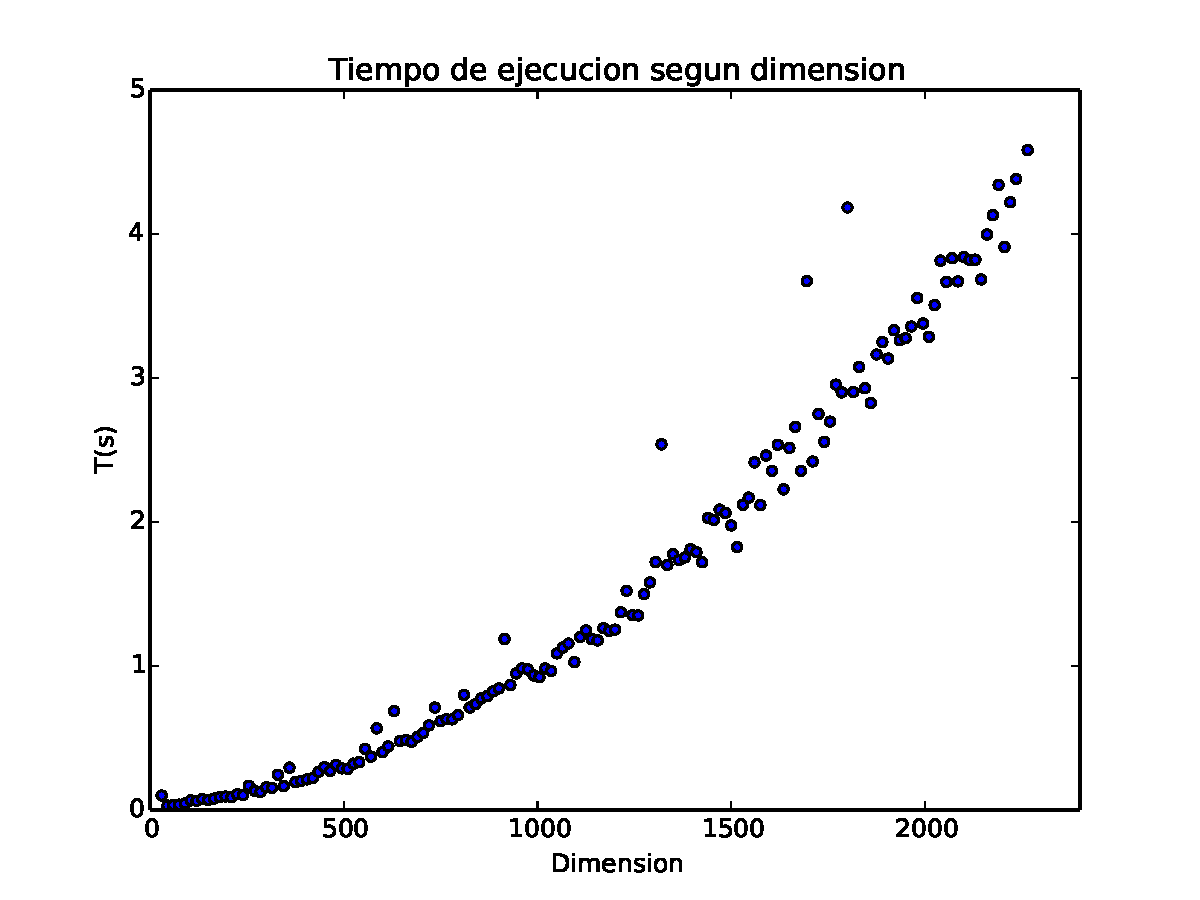
\includegraphics[scale=0.7]{images/complejidad.pdf}
\caption{A medida que aumenta c, muestra como cambia el ranking.}
\label{timePageRank}
\end{figure}